\documentclass[10pt,a4paper,twocolumn]{article}
\usepackage[a4paper,margin=17mm,columnsep=6mm]{geometry}
\usepackage[T1]{fontenc}
\usepackage{newtxtext,newtxmath}
\usepackage{microtype}
\usepackage{amsmath}
\usepackage{booktabs}
\usepackage{graphicx}
\usepackage{xcolor}
\usepackage[font=small,labelfont=bf,skip=4pt]{caption}
\usepackage{enumitem}
\usepackage[hidelinks]{hyperref}
\usepackage{tabularx}
\usepackage{array}
\setlist{nosep,leftmargin=*}
\graphicspath{{fig/}}
\newcommand{\Tab}[1]{\input{tab/tab_#1.tex}}
\newcommand{\NBcollhi}{6.9}
\newcommand{\NBmaxcoll}{6.9}
\newcommand{\NBmaxlat}{9.8}
\newcommand{\NBmaxlon}{7.1}
\newcommand{\NBmaxped}{7.1}
\newcommand{\NBmaxphi}{1.6}
\newcommand{\NBmaxtheta}{1.9}
\newcommand{\NBpowcorr}{3.6}
\newcommand{\NBpowfifty}{9}
\newcommand{\NBpowmax}{9}
\newcommand{\NBpowmin}{$-$6}
\newcommand{\NBthetahi}{1.9}
\newcommand{\NCmax}{10}
\newcommand{\NCmin}{2}
\newcommand{\NCratio}{9}
\newcommand{\NDownload}{2.3}
\newcommand{\NFMbemt}{0.010}
\newcommand{\NFMnorman}{0.026}
\newcommand{\NFMuniB}{0.028}
\newcommand{\NFe}{25.9}
\newcommand{\NGEmax}{0.006}
\newcommand{\NGEoge}{64.6}
\newcommand{\NHheavy}{0.948}
\newcommand{\NHmax}{0.995}
\newcommand{\NHmin}{0.965}
\newcommand{\NKc}{1.12}
\newcommand{\NKh}{1.06}
\newcommand{\NLcgmodel}{$-$0.98}
\newcommand{\NLcgtest}{$-$1.48}
\newcommand{\NLlaterr}{0.31}
\newcommand{\NLock}{8.1}
\newcommand{\NLrollerr}{1.4}
\newcommand{\NLswingmodel}{2.3}
\newcommand{\NLswingtest}{4.3}
\newcommand{\NMqgh}{$-$1.61}
\newcommand{\NMqmod}{$-$1.78}
\newcommand{\NMwgh}{0.0092}
\newcommand{\NMwmod}{0.0028}
\newcommand{\NProfilec}{43}
\newcommand{\NQgh}{19.3}
\newcommand{\NQmod}{17.4}
\newcommand{\NQtest}{24.1}
\newcommand{\NRbetter}{11}
\newcommand{\NRgh}{2.77}
\newcommand{\NRghhi}{106}
\newcommand{\NRghlo}{38}
\newcommand{\NRmhi}{47}
\newcommand{\NRmlo}{8}
\newcommand{\NRmod}{2.07}
\newcommand{\NRn}{16}
\newcommand{\NRped}{12}
\newcommand{\NSigma}{0.0821}
\newcommand{\NTRmax}{0.95}
\newcommand{\NTRmin}{0.89}
\newcommand{\NZqgh}{5.0}
\newcommand{\NZqmod}{$-$1.9}
\newcommand{\NZwgh}{$-$0.79}
\newcommand{\NZwmod}{$-$0.68}
\newcommand{\NaeroMB}{1.2}
\newcommand{\NnAftCG}{8}
\newcommand{\NnFcs}{380}
\newcommand{\NnFunc}{797}

\newcommand{\ok}{\textcolor{green!45!black}{\ensuremath{\checkmark}}}
\newcommand{\nok}{\textcolor{red!70!black}{\ensuremath{\times}}}
\newcommand{\pok}{\textcolor{orange!85!black}{\ensuremath{\sim}}}
\renewcommand{\arraystretch}{1.08}
\setlength{\tabcolsep}{4pt}
\raggedbottom
\renewcommand{\topfraction}{0.92}\renewcommand{\dbltopfraction}{0.92}\renewcommand{\bottomfraction}{0.6}
\renewcommand{\textfraction}{0.06}\renewcommand{\floatpagefraction}{0.85}\renewcommand{\dblfloatpagefraction}{0.85}
\setcounter{topnumber}{3}\setcounter{dbltopnumber}{3}\setcounter{totalnumber}{5}
\makeatletter\setlength{\@fptop}{0pt}\setlength{\@dblfptop}{0pt}\makeatother
\begin{document}

\twocolumn[
\begin{@twocolumnfalse}
\begin{center}
{\LARGE\bfseries Flight Dynamics of the Sikorsky UH-60A Black Hawk in JSBSim\par}
\vspace{6pt}
{\large\bfseries An individual-blade rotor model after Sikorsky's GenHel, checked against US Army flight tests\par}
\vspace{10pt}
{\large Technical report \quad\textbullet\quad October 2026\par}
\vspace{10pt}
\end{center}
\begin{abstract}
\noindent
A flight-dynamics model of the UH-60A Black Hawk for the FlightGear simulator has been written in JSBSim, replacing the
parametric YASim helicopter model the aircraft used before. It follows the structure of the Sikorsky General Helicopter
(GenHel) engineering simulation documented in NASA CR-166309: the four main rotor blades are simulated individually, each
with flap and lead-lag freedom, a nonlinear lag damper and eight aerodynamic segments using the SC1095 tables over
$\pm180^\circ$ and Mach number, under a Peters--He finite-state dynamic wake; the tail rotor is built the same way, with GenHel's
closed-form solution as the alternative, and the two are compared throughout; fuselage, stabilator and fin use GenHel's wind-tunnel tables,
and a ring-vortex wake decides how much of the main rotor's wake reaches the tail in any wind, and puts the fin in the tail rotor's wake; the automatic
flight control system (stabilator schedule, SAS, pitch bias actuator, flight path stabilization) and two T700 engines
with the rotor speed degree of freedom complete it. The whole model, \NnFunc{} aerodynamic functions and \NnFcs{}
control-system components, is generated by a script from transcribed data, and runs in plain JSBSim without scripting.
It was flown offline through a scripted programme and compared with US Army (USAAEFA) flight tests and with GenHel. Level-flight
trims from 50 to 162\,kt agree with the test within \NBmaxlon\,\% of longitudinal and \NBmaxcoll\,\% of collective travel
and \NBmaxtheta$^\circ$ of pitch attitude. Out-of-ground-effect hover power is \NHmin--\NHmax{} of the tethered-hover test,
rotor figure of merit is within \NFMnorman{} of the measured data, and ground-effect power savings are within \NGEmax{}.
For the 17 control-step responses of NASA TM-88360 the model's root-mean-square rate error is below GenHel's in \NRbetter{} of
\NRn{} usable cases (mean \NRmod{} against \NRgh\,deg/s). Hovering in winds from every direction, where GenHel's wash at the tail doubles
the pedal's swing, the ring wake brings the pedal error from \NXGped{} to \NXBped\,in rms. The hover pedal step exposed a missing term: the
rotor keeps its own angular momentum, so its speed relative to the airframe must follow the airframe's yaw; with that term the yaw-rate error
after the step fell from 5.5 to \NRpedrms\,deg/s. Deficiencies are quantified: cruise power 2--10\,\% above one
of two conflicting test sources, a weak pitch-up after an aft step at 100\,kt (\NQmod{} against \NQtest\,deg/s), an angle-of-attack
derivative $M_w$ a third of that of TM-85890's model, half the bank change between climb and descent that the aircraft shows, and a tail
rotor that reaches its stall near the top speed, where the aircraft still had pedal to spare.
\end{abstract}
\vspace{6pt}
\end{@twocolumnfalse}
]

% =====================================================================================================================
\section{Introduction}
The UH-60A distributed for FlightGear flies on YASim, whose helicopter model builds the rotor from a short list of geometric
parameters and tuning factors. Its behaviour is set by tuning rather than by the aircraft's data, and its couplings, power
characteristics and responses cannot be traced to measurements. For the UH-60A, unusually,
the data exist in public: in the early 1980s Sikorsky documented its General Helicopter (GenHel) engineering simulation of
the Black Hawk in full for NASA~\cite{gh}, NASA re-implemented and validated it against US Army flight tests~\cite{hb,bal},
and the Army's test reports~\cite{a7717,a7924,a8324} give trim, stability and performance data for the same airframes.

This report describes a JSBSim~\cite{jsbsim} model built on that material and how well it reproduces the tests. GenHel is used
as the blueprint, not as gospel: where it leaves the physics incomplete (the induced power, Section~\ref{sec:power}) or where
validation exposed an inconsistency, the model departs from it, and the departures are listed in Section~\ref{sec:review}.
All of the flight model, including the rotor's integration, the control laws and the engines, is JSBSim XML; the FlightGear side
only animates and instruments it. All result tables, and the numbers quoted from them, are written by the evaluation scripts.

% =====================================================================================================================
\section{Reference data}\label{sec:ref}
\begin{table}[t]
\centering\small
\caption{Sources and what they contribute.}\label{tab:sources}
\begin{tabularx}{\columnwidth}{@{}>{\raggedright\arraybackslash}p{2.55cm}X@{}}
\toprule
Source & Content used \\
\midrule
NASA CR-166309~\cite{gh} & GenHel: rotor, tail rotor, fuselage, empennage, controls, AFCS, engine equations; SC1095, fuselage and empennage tables; physical and mass data \\
NASA TM-85890~\cite{hb} & parameter tables, control rigging and mixing; stability derivatives of its own (simpler, rotor-map) model \\
NASA TM-88360~\cite{bal} & level-flight trims vs.\ airspeed (fig.~B1); 17 control-step responses (app.~D) with test conditions (table~C1) \\
NASA CR-177360~\cite{kap} & GenHel against Army tests: sideslip sweeps; tail-rotor wash on the fin \\
USAAEFA 79-24~\cite{a7924} & the test behind TM-88360: inherent sideslip, lateral-directional sweeps, static and long-term stability; fin and stabilator dimensions \\
USAAEFA 77-17~\cite{a7717} & tethered hover, tail rotor shaft power, level-flight power (first-year aircraft); low speed in every wind direction (figs.~106--110) \\
USAAEFA 83-24~\cite{a8324} & hover fits of 77-17 reanalysed, sixth-year aircraft with ESSS fairings \\
DTIC ADA180404~\cite{a85} & sideslip in climbs and descents \\
NASA TP-2003-212265~\cite{bous} & SC1095 geometry, tip sweep, drag at full-scale Reynolds number, tripping increment \\
LRTA paper~\cite{lrta} & UH-60 rotor figure of merit from flight and wind tunnel tests \\
JAHS 2004 paper~\cite{perf} & accessory power; flat-plate drag area; tail rotor power of the Airloads flights \\
NASA TM 110362~\cite{flet} & hover derivatives identified from flight test; rotor speed equation \\
DTIC ADA181947~\cite{a87} & inherent sideslip with the ESSS fairings \\
USAAMRDL TR 72-67~\cite{gorm} & dynamic stall delay (tail rotor experiment) \\
NASA TN D-234~\cite{heyson} & ground effect in forward flight \\
METU thesis~\cite{metu} & Peters--He finite-state wake equations \\
TM 1-1520-237-10~\cite{tm} & hover chart (ground effect, power), limits, procedures, AFCS functions, tail rotor construction \\
NASA T700 study~\cite{t700} & engine and fuel control dynamics \\
\bottomrule
\end{tabularx}
\end{table}

Table~\ref{tab:sources} lists the sources; most are scans, and every curve used was digitised from them. A few points of
data reduction matter for the comparisons.
\emph{(i)} The control-step responses of TM-88360 were digitised from 68 plot pages (some scanned sideways or upside down);
each case is replayed at its own test condition from table~C1 of that report: weight, centre of gravity (CG), density
altitude and speed. \NnAftCG{} of the cases, all five in hover among them, were flown at FS\,359.2--359.6, near the aft limit; for the aft step at
100\,kt this raises the pitch response by half.
\emph{(ii)} The trims of TM-88360 fig.~B1 come from USAAEFA test 79-24; its own figure~1 shows that the three points plotted at
22--32\,kt were flown at 3--15\,KCAS, so they are near-hovers and are shown apart.
\emph{(iii)} Two tests of the same airframe, S/N 77-22716, disagree on cruise power: at 95\,kt the main rotor torque of 79-24
(TM-88360) implies 4--6\,\% more power than the engine torque of 77-17, of which instrumentation drag explains about 2\,\%.
\emph{(iv)} The hover charts of the operator's manual represent the sixth-year aircraft with the external stores support system
(ESSS) fairings, which needs about 3\,\% more hover power than the first-year aircraft; the model is compared with the latter.

% =====================================================================================================================
\section{The model}\label{sec:model}
\begin{figure*}[t]
\centering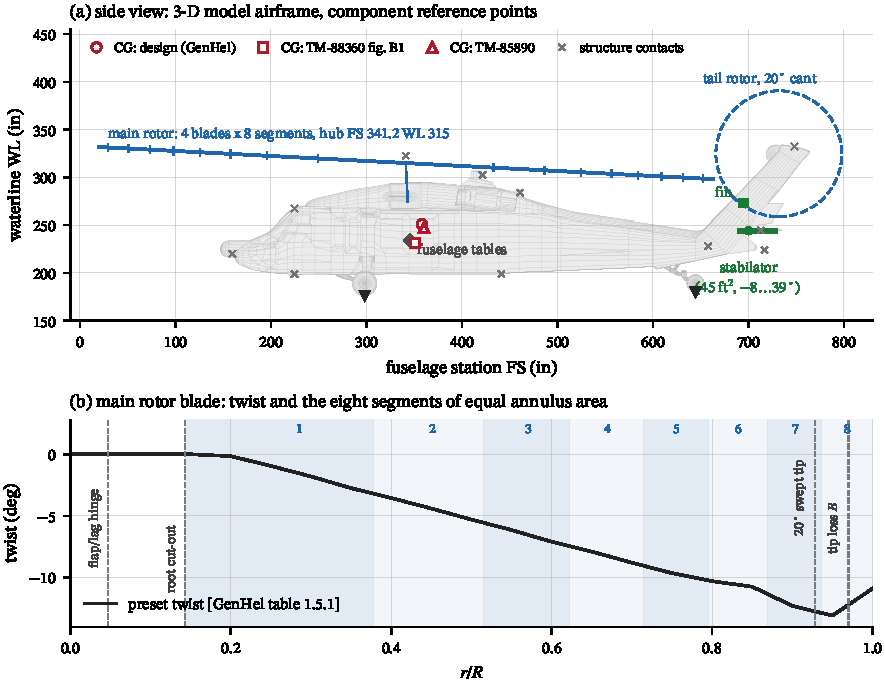
\includegraphics[width=\textwidth]{geometry.pdf}
\caption{Geometry. (a) The FlightGear 3-D model's airframe in Sikorsky stations, with the main rotor disc (3$^\circ$ forward shaft tilt;
ticks at the segment mid-points), the tail rotor, the stabilator and fin reference points, the reference point of the fuselage tables, the three
centres of gravity used in this report, the wheels ($\blacktriangledown$) and the 17 structure contacts. (b) The main rotor blade: preset twist and the
eight segments of equal annulus area.}\label{fig:geometry}
\end{figure*}

\subsection{Implementation}
A Python script writes the model from the transcribed tables (Table~\ref{tab:model}). JSBSim evaluates aerodynamic functions on
demand, so the function graph must be free of cycles; every quantity that depends on its own past, the blade flap and lag
angles and rates of both rotors, the wake states, the rotor speed, the tail rotor inflow, the blade's elastic twist and the engines' states,
therefore lives in flight-control-system channels, which JSBSim runs once per frame in a fixed order and which can write
properties back. These channels integrate the states explicitly at the simulation rate of 480\,Hz, which is
3.2$^\circ$ of rotor azimuth per step; the wake states use a semi-implicit step. Trims and control responses at this rate
are within 0.5\,\% of those at 960\,Hz, where 120\,Hz was off by up to 4\,\%, and one step costs about 0.1\,ms. The blade loads of a frame use the states of
the previous frame. The same XML runs in FlightGear and in the offline harness used here.

\begin{table}[t]
\centering\small
\caption{The generated model: JSBSim system files, their content and the number of control-system components or named
aerodynamic functions.}\label{tab:model}
\Tab{model}
\end{table}

\subsection{Main rotor}
Each blade is a rigid beam on a coincident flap and lag hinge at 4.66\,\% radius. Its eight segments of equal annulus area
(Fig.~\ref{fig:geometry}b) see the air velocity at their mid-point from the full kinematics in shaft axes: the aircraft's
translation and rotation, the rotor speed, the blade's flap and lag motion and the induced velocity. Lift and drag come from the
SC1095 tables of GenHel against angle of attack ($\pm180^\circ$; the drag of the reversed section near $180^\circ$, which GenHel's
table sets to zero, is restored) and Mach number, which on the 20$^\circ$ swept tip is that of the velocity normal to the leading edge. Lift acts on the
velocity normal to the span; drag acts along the whole flow including its spanwise part, which is what gives the blade's profile power its
growth with advance ratio. A section drag increment of 0.0012 is added to the smooth wind-tunnel tables: a production blade's boundary layer is turbulent from
near the leading edge, and tripping added about half of the NACA 0012 increment~\cite{nacaexp} to the SC1095 at full-scale Reynolds
number~\cite{bous}. GenHel's empirical torsional wind-up twists the tip nose-down in proportion to the mean blade load.
The tip loss factor $B=0.97$ removes the lift outboard of $B R$ and, unlike GenHel, also enters the momentum balance
(Section~\ref{sec:power}).

The flap equation of each blade contains the aerodynamic hinge moment, the hub's specific force, the gyroscopic terms
from the body's rate and acceleration, the centrifugal stiffness (including the lead rate) and the lag damper; the blade rests
on droop and anti-flap stops. The lag equation contains the aerodynamic and damper moments, the centrifugal stiffness of the
hinge offset, the Coriolis moment of flapping and the rotor's acceleration. The lag damper's force comes from GenHel's
force--stroke-speed table and acts through the geometry of its two pickups, one on the hub and one on the blade cuff, which
turns with blade pitch, so that its flap and lag moments follow from virtual work. The blades' aerodynamic and inertial loads act on the hub at their hinges; the
shaft torque drives the rotor speed.

\subsection{Inflow}
The induced velocity comes from the Peters--He generalised dynamic wake~\cite{metu} with three axisymmetric states, giving the
radial distribution in hover, and the first harmonic pair, driven by the rotor's hub moments and coupled to the wake skew. Its
inflow gain matrices are tabulated against the wake skew parameter. The states are kept in the hub frame and turned into the
frame of the in-plane flow for their update, so that a wake that swings round with the flow direction in a hover does not
carry the states with it. Ground effect scales the induced velocity: in hover by $(1+0.3(R/Z)^2)^{-1/2}$, with $Z$ the height
of the hub, which reproduces the power savings of the operator's manual hover chart~\cite{tm} (GenHel's own form gives half of them), and in
forward flight by the ratio of forward-flight to hover interference of TN D-234~\cite{heyson} against the angle of the wake.
For use in the simulator, coloured noise can be added to the inflow and its gradients in the regimes where the real wake is
unsteady (ground effect, translational lift, vortex ring); its intensities are estimates and it is off in all results here.

\subsection{Tail rotor}
Two tail rotor models can be built from the same data; both are compared in Section~\ref{sec:results}. Both are canted
20$^\circ$ so that the rotor also lifts, take GenHel's rigging from the pedals (with the collective mixing) to the pitch at the
blade cuff, and see the same air at the hub.

\emph{GenHel's closed form.} Bailey's solution for a rotor with linear twist~\cite{gh} gives the thrust and torque coefficients in
terms of the inflow and advance ratios, with pitch--flap coupling ($\tan\delta_3=0.70$) through the coning per pound of thrust, a tip
loss of 0.92 and the inflow solved by a relaxed fixed-point step per frame over the effective disc. Its pitch is the cuff angle plus
GenHel's 6$^\circ$ ``blade pitch correction to linear twist'': with the $-18^\circ$ twist, the linear blade has the cuff's pitch at a third
of the radius. Lift stays linear in the angle of attack, without stall or reversed flow, and terms above $\mu^2$ are dropped.

\emph{Blade-element rotor.} The second model is built like the main rotor. Four blades flap on a hinge at the centre, for the bearingless
crossbeam whose graphite spars run from tip to opposite tip~\cite{tm}; their flap inertia follows from the Lock number (3.38) and a weak
spring stands for the spars' stiffness, which is not published (flap frequency 1.02 per revolution, in keeping with GenHel's coning per
pound of thrust). Each blade's pitch is the closed form's, less $\tan\delta_3$ times its own flapping. Six segments from 0.2\,$R$ use the SC1095
tables against angle of attack ($\pm180^\circ$) and Mach number in the air at the hub plus the blade's own motion and a uniform dynamic inflow
(Pitt--Peters momentum over the effective disc), which reverses with the thrust and is not limited in the vortex ring state. The thrust,
in-plane forces and hub moments, the drive torque among them, come from the blades.

\emph{Air at the tail rotor.} GenHel computes it ``in the same manner as the empennage''~\cite{gh}: with the stabilator's and fin's main
rotor wash factors, which depend on the wake's skew and the disc's tilt but not on the direction the wake is blown, so that the far wake's
twice-mean induced velocity reaches the tail rotor in any wind. The tail rotor hub is 1.21\,$R$ behind the main rotor's and 0.8\,ft above it:
at the upper edge of the wake when that is blown aft, clear of it when it is blown sideways or forward. The model takes the main rotor's
induced velocity at the tail rotor from a skewed cylinder of ring vortices (uniform loading, the wake of TN D-234~\cite{heyson}) leaving the
tip-path plane, averaged over the tail rotor's disc and tabulated against the skew, the direction of the in-plane flow and the longitudinal
flapping (Fig.~\ref{fig:wake}a). The fuselage's sidewash and the dynamic-pressure loss of the fin maps are GenHel's.

\emph{Fin blockage.} The tail rotor is a tractor whose wake meets the fin. GenHel multiplies the thrust by 0.796 in the hover, fading to 1 by
30\,kt in any wind direction. Here the tail rotor's own ring wake, skewed by the flow through and along its disc, gives the induced velocity
over four spanwise strips of the fin (the planform of the principal dimensions~\cite{a7924}), and the blockage is the fin's own lift and drag in
it: largest in the hover and with the wind from the right, which blows the wake onto the fin; small with the wind from the left, which blows it
back through the rotor; a few per cent of the thrust in cruise. The ring wake puts 13.6\,\% of the hover thrust on the fin, where Sikorsky
measured 20.4\,\% (GenHel's 0.796), and it is used as it is. Scaled up to Sikorsky's figure (by 1.25 in velocity) the jet at the fin, only
0.2\,$R$ behind the disc, would be close to its far-wake speed, and the fin would give back more of the rotor's yaw damping than the rotor
loses to it (Section~\ref{sec:resp}).

\begin{figure}[t]
\centering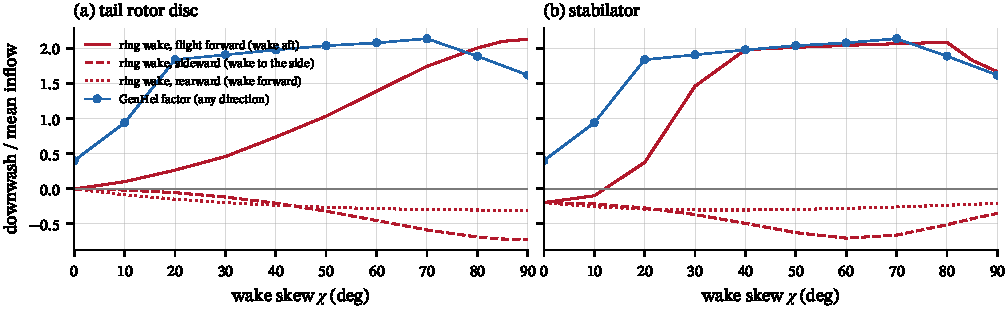
\includegraphics[width=\columnwidth]{wake.pdf}
\caption{Main rotor downwash, over its mean inflow, (a) over the tail rotor's disc and (b) over the stabilator: the ring wake for the aircraft
flying forward, sideward and rearward (level disc, $a_1=0$), and GenHel's interference factor, which applies in any direction.}\label{fig:wake}
\end{figure}

\subsection{Airframe}
The fuselage forces and moments come from GenHel's tail-off wind-tunnel tables against angle of attack and sideslip, evaluated
with the local flow that includes the main rotor wake through GenHel's interference factors (functions of the wake skew and
the disc's tilt). In rearward flight the tables are mirrored front to back. The stabilator and fin are strips with their own
lift and drag tables over $\pm180^\circ$, the rotor wake, the fuselage's downwash, sidewash and dynamic-pressure loss at the
tail. At the stabilator the ring wake reproduces GenHel's downwash factor, measured with the wake blown aft, from 40$^\circ$ of skew up
(Fig.~\ref{fig:wake}b); GenHel's factor is kept and the ring wake adds how the downwash changes when the wake is blown sideways or
forward. The fin's in-plane wash comes from the ring wake over its planform. GenHel's empirical downwash correction terms~\cite{gh}, a side
force, a rolling moment and a sideslip-dependent pitching moment for the wake's swirl at the empennage, from rotor-on wind tunnel tests and
flight test, complete the airframe.

\subsection{Flight controls}
The rigging and the mechanical mixing (collective to cyclic and pedal, pedal to longitudinal cyclic) follow TM-85890~\cite{hb}; the
primary servos are second-order systems. The automatic flight control system is GenHel's: the stabilator scheduled on airspeed and
collective with pitch rate and lateral acceleration feedback; the two stability augmentation channels (SAS\,1 analogue,
SAS\,2 digital, 10\,\% authority together); the pitch bias actuator; and the flight path stabilization (FPS) with attitude,
airspeed and heading hold and turn coordination through the trim actuators. FlightGear cannot move the pilot's stick, so the
FPS moves the stick's trim point instead, and the pilot's trim release becomes automatic when a control moves away from it.
The tail rotor rigging carries 0.5\,in of left pedal that GenHel's rigging lacks: TM-88360 found GenHel ``a nearly constant pedal bias of
approximately 0.5\,in.\ to the right'' of the flight test in level flight. CR-177360 obtained a similar shift at 140\,kt by putting
1.2 times the tail rotor's induced velocity on the fin, but judged the factor unsubstantiated; with the fin in the tail rotor's ring wake the
model finds that interaction at a few per cent of the thrust in cruise, so the offset is kept as rigging.

\subsection{Engines, drive and mass}
Each T700-GE-700 is modelled after GenHel's engine module and the NASA integration study~\cite{t700}: the hydromechanical
unit meters fuel within acceleration and deceleration schedules to hold a gas generator speed reference from the power lever or the
collective's load-demand spindle, trimmed by the power-turbine speed governor; the gas generator follows with its speed-dependent
lag and the power turbine's torque depends on both speeds. Freewheel clutches connect the engines to the main gearbox; the rotor speed
is a degree of freedom with the inertia of hub, drive and blades. The blades' share, 6970\,slug\,ft$^2$ about the shaft (a fifth of the
airframe's yaw inertia), keeps its own angular momentum: the rotor's speed relative to the airframe changes by the airframe's yaw
acceleration about the shaft~\cite{flet}, so a yaw droops or speeds the rotor, the tail rotor with it, and the governor's answer reaches the
airframe as the drive torque's reaction. The gearbox absorbs 3\,\% of the main rotor torque (assumed) and the
accessories 65.8\,hp, Sikorsky's figure~\cite{perf}. Table~\ref{tab:params} lists the principal data. The default loading is
GenHel's design point; each validation case uses its own test loading. The landing gear has two main wheels and a castering tail
wheel; 17 structure contacts taken from the 3-D model's skin carry the aircraft when it lands on its belly or rolls over.

\begin{table}[t]
\centering\small
\caption{Principal data.}\label{tab:params}
\Tab{params}
\end{table}

% =====================================================================================================================
\section{Method}\label{sec:method}
The evaluation drives JSBSim from Python with the same files as FlightGear, at 480\,Hz, with the wake noise off. A trim solves for
the four controls and the attitudes that zero the six accelerations averaged over two rotor revolutions (Hann-weighted, so that the
tail rotor's 4.6 revolutions per main rotor revolution leave no phase-dependent remainder), with the airframe held while the rotor and
wake settle. Away from the nose the trim variables are the pitch and roll attitudes with the velocity fixed in the earth frame, since
angle of attack and sideslip lose their meaning at 90$^\circ$ off the nose. Atmospheres reproduce each test's pressure and density altitude (JSBSim's temperature
offset and the geometric altitude are iterated). The programme:
\begin{itemize}
\item \emph{Level-flight trims} from hover to 162\,kt at the loading of TM-88360 fig.~B1 (16\,000\,lb, FS\,351, WL\,231.5, 5250\,ft);
\item \emph{lateral-directional trims}: zero-sideslip and wings-level trims at 60, 100 and 140\,kt, in 1500\,fpm climbs and descents
and with the CG 2.1\,in right and 4.1\,in left, against the digitised sweeps of 79-24 and ADA180404;
\item \emph{power}: out-of-ground-effect hover from 11\,000 to 22\,000\,lb at the 2302\,ft test site; level flight at $C_T\times10^4$
= 65 to 90 and $\mu$ = 0.10 to 0.32; the isolated rotor's figure of merit at sea level; and blade-element momentum calculations of
the same blade as a reference;
\item \emph{ground effect}: the test autopilot (written for the FlightGear flight tests) hovers the model at 5, 10, 20, 40 and 100\,ft
wheel height;
\item \emph{control responses}: the recorded control increments of the 17 cases of TM-88360 app.~D, applied open loop from a
trim at the test condition with the SAS, FPS and pitch bias actuator off and the stabilator fixed, as in the test;
\item \emph{stability derivatives} at 100\,kt at the loading of TM-85890 (16\,400\,lb, FS\,360.4), by central differences of the
aerodynamic forces with the airframe held;
\item \emph{low speed in every wind direction}: trims at 10, 20, 30, 35 and 40\,KTAS and relative wind azimuths from 0 to 360$^\circ$ at
25\,ft wheel height, at the conditions of the two aircraft of 77-17 figs.~106--110 (16\,880\,lb at 9860\,ft and 16\,330\,lb at 2080\,ft
density altitude, forward CG; weights from the plotted $C_T$), against their pedal, longitudinal cyclic and tail rotor shaft power;
\item \emph{tail rotor power in level flight} against the UH-60A Airloads flights 84--90~\cite{perf} at main rotor weight coefficients
$C_W$ = 0.0065 to 0.0091, wings level as flown and at 5$^\circ$ of nose-left sideslip, 16\,500\,lb at the density giving each $C_W$;
\item \emph{hover yaw derivatives}, quasi-static and by component, at the hover of the pedal step and at the 1-kt condition of TM-85890.
\end{itemize}
Each tail-rotor-related stage is run with both tail rotor models, and the crosswind trims also with GenHel's wash factors at the tail.

% =====================================================================================================================
\section{Results}\label{sec:results}
\subsection{Level-flight trim}
\begin{figure*}[t]
\centering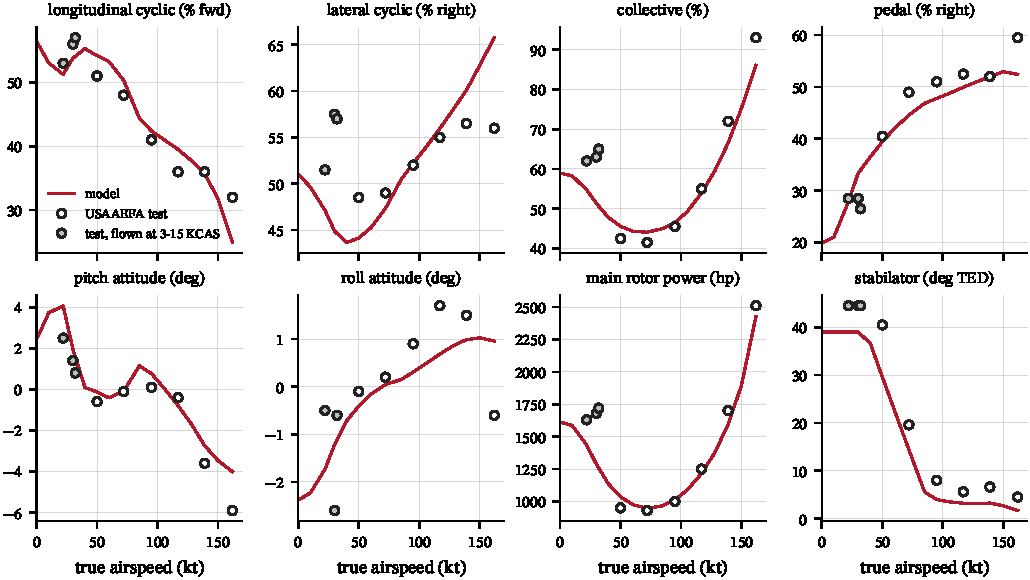
\includegraphics[width=\textwidth]{trim.pdf}
\caption{Level-flight trim against the USAAEFA test of TM-88360 fig.~B1: 16\,000\,lb, FS\,351, 5250\,ft density altitude. Grey
symbols: points plotted at 22--32\,kt but flown at 3--15\,KCAS. Controls are in per cent of travel; power is the main rotor's.}\label{fig:trim}
\end{figure*}

\begin{table}[t]
\centering\small
\caption{Level-flight trim: model minus test (TM-88360 fig.~B1); power as model/test $-1$. $^*$Flown at 3--15\,KCAS.}\label{tab:b1}
\Tab{b1}
\end{table}

Figure~\ref{fig:trim} and Table~\ref{tab:b1} compare the trims. From 50 to 162\,kt the longitudinal cyclic is within
\NBmaxlon\,\% of its travel, the collective within \NBmaxcoll\,\%, the pitch attitude within \NBmaxtheta$^\circ$ and the roll attitude within
\NBmaxphi$^\circ$. Main rotor power is within \NBpowmin{} to $+$\NBpowmax\,\%, the largest excess at 50\,kt; the model
reproduces the test's 930--950\,hp minimum between 50 and 95\,kt only from 72\,kt up. The pedal is \NBpedmin{} to \NBpedmax\,\% of travel from
the test between 50 and 139\,kt with the blade-element tail rotor and \NBYpedmin{} to \NBYpedmax\,\% with Bailey's. The largest
differences are at 162\,kt: the collective \NBcollhi\,\% low, the lateral cyclic \NBmaxlat\,\% right of the test, the nose
\NBthetahi$^\circ$ high, and the pedal \NBpedhs\,\% from the test, which moves 7.5\,\% to the right between 139 and 162\,kt. That move is the
collective-to-pedal mixing: the collective rises by a fifth of its travel, and through the rigging the test's tail rotor pitch goes from
\NBtrpTlo{} to \NBtrpThi$^\circ$ (+\NBtrpTrise$^\circ$), against \NBtrpYlo{} to \NBtrpYhi$^\circ$ (+\NBtrpYrise$^\circ$) for Bailey's rotor
(\NBYpedhs\,\% of pedal from the test). The blade-element rotor, asked for some 1600\,lb at an advance ratio of 0.4, reaches the static
stall of its retreating blades near 17.5$^\circ$: more pitch no longer adds thrust, and the trims stop short of a balance from about 158\,kt.
Its sections pitch there at a reduced frequency near 0.2, where real sections stall later. Gormont's dynamic stall delay~\cite{gorm},
built in as a switch, leaves the trims below the stall unchanged. With its reattachment delay applied once a section has stalled, the limit
stays where it is; without it the 162\,kt point trims, at 19.3$^\circ$ and 1780\,lb, the main rotor at 2600\,hp against the test's 2510. The crossbeam's flap stiffness, which is
not published, also moves the limit (with a flap frequency of 1.15 per revolution instead of 1.02 the point trims). Over the scatter of the
pedal readings (about 1$^\circ$ of tail rotor pitch) the model follows the test's pitch from 95 to 139\,kt; the test's small rise to 162\,kt,
with the main rotor's torque up by half, points to anti-torque the model lacks at the top speed. The near-hover test points need 7--14\,\% more collective than the model at 22--32\,kt and 3--4\,\% more than its
hover at 1\,kt; there the stabilator's schedule saturates at the model's 39$^\circ$ limit, where the test reads 44.5$^\circ$.

\subsection{Lateral-directional trim}
\begin{table*}[t]
\centering\small
\caption{Lateral-directional trim against USAAEFA 79-24 sweeps (zero sideslip, from the sweep through it) and ADA180404.
Lateral cyclic in inches from full left, pedal in per cent of travel from full left.}\label{tab:latdir}
\Tab{latdir}
\end{table*}

At zero sideslip (Table~\ref{tab:latdir}) the model's lateral cyclic is within \NLlaterr\,in of the test and its bank within
\NLrollerr$^\circ$. GenHel's downwash correction terms matter here: without them the model trimmed at up to 2.5$^\circ$ of left bank,
a side force of some 900\,lb missing near the CG at 100\,kt, which neither the tail rotor nor the rotor's tilt can supply. Two effects
are only partly reproduced: the bank swings by \NLswingmodel$^\circ$ between a 1500\,fpm descent and a climb against \NLswingtest$^\circ$ in
the test, and moving the CG from BL\,$-4.1$ to $+2.1$\,in costs \NLcgmodel\,in of lateral cyclic against \NLcgtest\,in, so the
model's roll moment per inch of cyclic is about 1.5 times too large, or the test's lateral CG shift smaller than its loading implies.

\subsection{Low speed in every wind direction}\label{sec:xwind}
\begin{figure*}[t]
\centering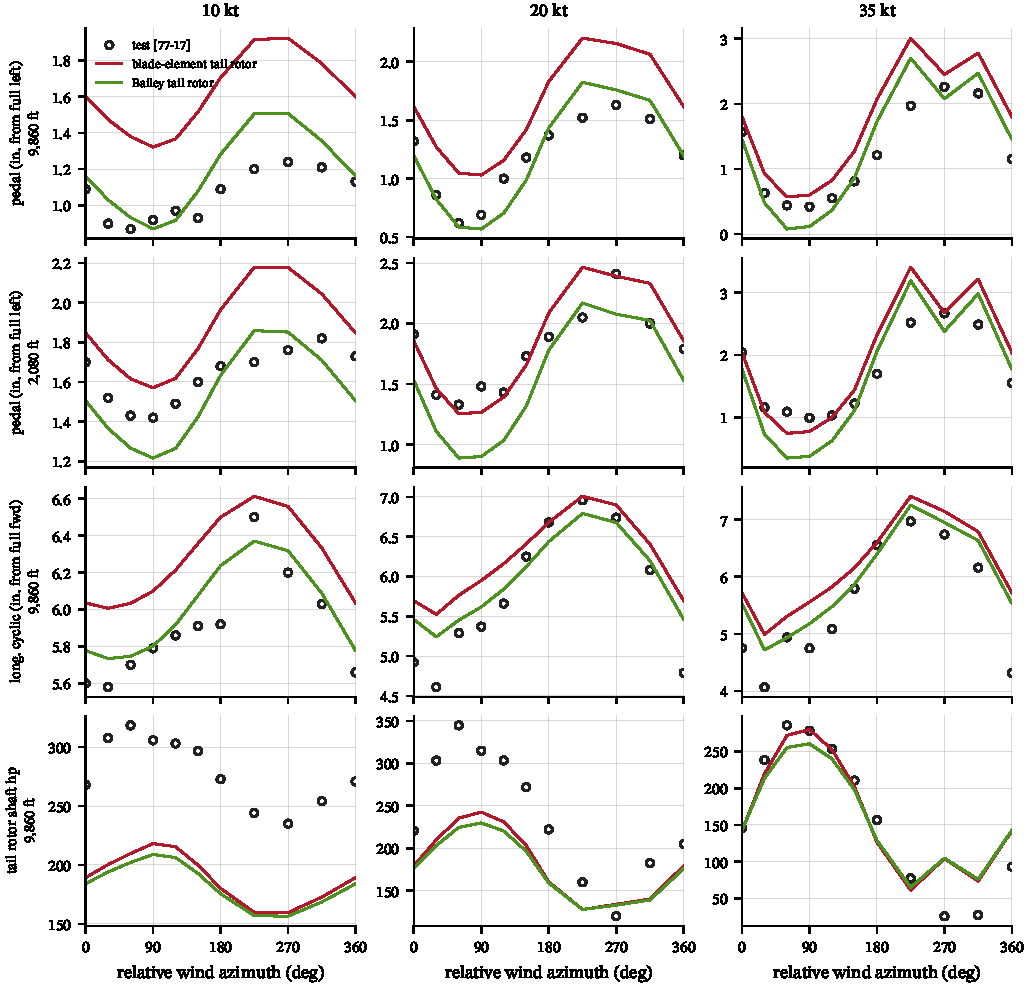
\includegraphics[width=\textwidth]{xwind.pdf}
\caption{Low speed in every wind direction, 25\,ft wheel height, against USAAEFA 77-17 figs.~106--110: pedal of both aircraft (716 at 9860\,ft,
717 at 2080\,ft density altitude), longitudinal cyclic and tail rotor shaft power of 716, with both tail rotor models. Relative wind azimuth from the
nose, clockwise: 90$^\circ$ is the wind from the right (right sideward flight), 180$^\circ$ rearward flight.}\label{fig:xwind}
\end{figure*}
\begin{table}[t]
\centering\small
\caption{Low speed in every wind direction (77-17 figs.~106--110, 10--40\,KTAS; aircraft 716 at 9860\,ft, 717 at 2080\,ft): model minus test over
all azimuths and speeds, with GenHel's wash factors at the tail, and with the ring wake and either tail rotor.}\label{tab:xwind}
\Tab{xwind}
\end{table}
Hovering in a wind is where the tail rotor works hardest and where its air is least like the free stream. In the 77-17 tests
(Fig.~\ref{fig:xwind}, Table~\ref{tab:xwind}) the aircraft needs the most left pedal with the wind from the right front, its critical azimuth,
where only 0.5\,in of pedal remained at 35\,KTAS, and the most right pedal with the wind from the left; its tail rotor takes 340\,hp at
60$^\circ$ and 25\,hp at 270$^\circ$. With GenHel's wash factors at the tail the model has this shape but swings nearly twice as far, and runs
out of left pedal at 35--40\,KTAS: its tail rotor meets the far wake's downwash and, in sideward flight, a crosswind 1.4 times the real one.
With the ring wake at the tail and the fin in the tail rotor's own wake, the pedal error falls from \NXGped{} to \NXBped\,in rms with the
blade-element rotor (\NXYped\,in with Bailey's) and the longitudinal cyclic error from \NXGlon{} to \NXBlon\,in. The blade-element rotor keeps
pedal in reserve throughout, 0.4\,in at the least, as the aircraft did; Bailey's, less effective per degree, runs out at 40\,KTAS with the
wind from the right front. With the fin's blockage as the ring wake gives it (13.6\,\% of the hover thrust, Section~\ref{sec:model}) the
blade-element rotor's pedal lies \NXBpedmeanC\,in right of the 716 aircraft's on average, the high-altitude one. The tail rotor's shaft power is \NXBtrhpC\,hp rms from the test's, lowest against it with the wind from the right front; the pedal remains
furthest to the right of the test with the wind from behind and from the left rear.

\subsection{Power}\label{sec:power}
\begin{figure*}[t]
\centering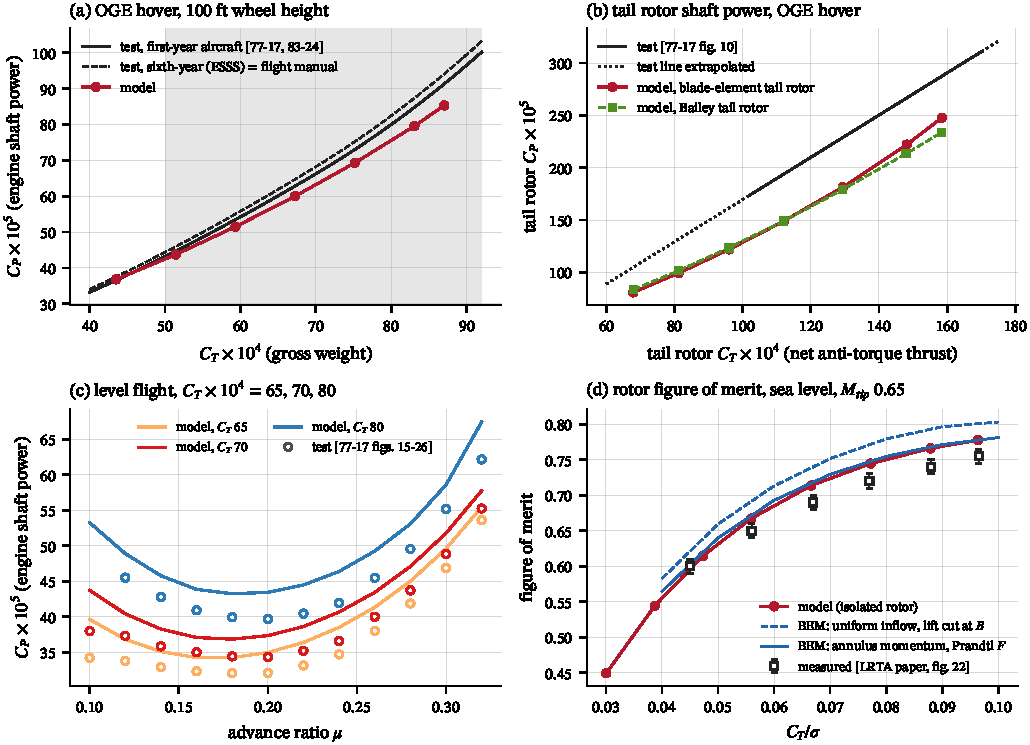
\includegraphics[width=\textwidth]{power.pdf}
\caption{Power. (a) Out-of-ground-effect hover at the 2302\,ft test site against the tethered-hover fits of 83-24 (shaded: test data range). (b) Tail rotor
shaft power in the same hovers against 77-17 fig.~10. (c) Level flight against the faired data of 77-17 figs.~15--26 at 263 referred rpm.
(d) Figure of merit of the isolated rotor, with two blade-element momentum (BEM) calculations of the same blade.}\label{fig:power}
\end{figure*}

\begin{table}[t]
\centering\small
\caption{OGE hover: model against the first-year aircraft's tethered-hover fit~\cite{a8324}; tail rotor against 77-17 fig.~10 (bracketed: outside its data).}\label{tab:hover}
\Tab{hover}
\end{table}

GenHel applies the tip loss factor to the blade lift only. Its inflow is the momentum solution for the full disc, so the
induced power it computes is ideal. The physical counterpart of the lost lift near the tip is a wake carried by the effective
disc $B^2 A$~\cite{johnson}: the induced velocity is $1/B$ times the full-disc value in hover and $1/B^2$ edgewise. The model applies this to
both rotors by scaling the Peters--He forcing, and the tail rotor's momentum term, by $1/B^2$. The isolated rotor's figure of merit
(Fig.~\ref{fig:power}d) then lies within \NFMbemt{} of a blade-element calculation with annulus momentum and Prandtl's distributed tip
loss, and within \NFMnorman{} of the measured values; with the lift cut alone it is \NFMuniB{} higher.

The complete aircraft (Fig.~\ref{fig:power}a, Table~\ref{tab:hover}) needs \NHmin--\NHmax{} of the measured engine power in the
range of the test data and \NHheavy{} at 22\,000\,lb; the deficit grows with thrust. The tail rotor needs \NTRmin--\NTRmax{} of
its measured shaft power. In level flight (Fig.~\ref{fig:power}c) the model needs \NCmin{} to \NCmax\,\% more power than the 77-17
data, \NCratio\,\% at $\mu=0.22$, while its main rotor power agrees with the 79-24 measurements of the same airframe
(Table~\ref{tab:b1}) within \NBpowcorr\,\% from 72\,kt up once the latter's instrumentation drag (2.8\,ft$^2$~\cite{perf}) is allowed for. The power budget (Table~\ref{tab:budget}) shows
nothing out of the ordinary: the airframe's drag area of \NFe\,ft$^2$ matches Sikorsky's 25.7\,ft$^2$~\cite{perf}, induced power
factors are \NKh{} in hover and \NKc{} in cruise, and the blades' profile drag is \NProfilec\,\% of main rotor power at
$\mu=0.22$, from section drag coefficients that agree with the SC1095 polars~\cite{bous}. The pattern that remains, too little power in
hover and too much in cruise against 77-17, survives any choice of the drag increment; it is the largest unexplained item of
the model. The hover download is \NDownload\,\% of weight, for which no UH-60 measurement was found.

\begin{table}[t]
\centering\small
\caption{Power budget: OGE hover at 17\,000\,lb (2302\,ft site) and level flight at $C_T=0.0070$ (5250\,ft).}\label{tab:budget}
\Tab{budget}
\end{table}

\subsection{Tail rotor power in level flight}
\begin{figure*}[t]
\centering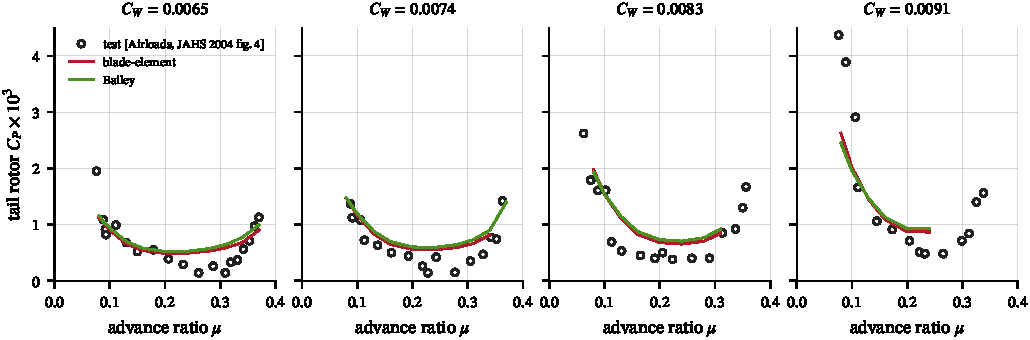
\includegraphics[width=\textwidth]{trpower.pdf}
\caption{Tail rotor shaft power in level flight, wings level, against the UH-60A Airloads flights at four main rotor weight coefficients, with both
tail rotor models. $C_P$ of the tail rotor on its own disc and tip speed.}\label{fig:trpower}
\end{figure*}
The Airloads flights measured the tail rotor's power from the intermediate shaft torque (Fig.~\ref{fig:trpower}). Here the model needs
more than the test: from $\mu$ = 0.12 to 0.20, \NTPBlom$\times10^{-3}$ against \NTPBlot$\times10^{-3}$ (Bailey's rotor \NTPYlom), and in cruise,
$\mu$ = 0.22 to 0.32, \NTPBmidm$\times10^{-3}$ against \NTPBmidt$\times10^{-3}$, where the measured value lies below what the blades' profile drag
alone should take ($\approx 0.3\times10^{-3}$ for a mean section drag coefficient of 0.0095). From $\mu$ = 0.33 up the measured power rises steeply;
Bailey's rotor follows it at \NTPYhi{} times, while the blade-element rotor reaches its thrust limit at the heavier weights, as at 162\,kt.
The excess in forward flight is the opposite of the hover, where the model's tail rotor needs less than the 77-17 aircraft; the Airloads aircraft
was a sixth-year one with the ESSS fairings. The comprehensive analysis of the same flights~\cite{perf}, with a free wake, also exceeds the
measurement in cruise and comes closer with 5$^\circ$ of nose-left sideslip. The flights were flown wings level, which takes some sideslip,
and the ESSS fairings add 2--3$^\circ$ of nose-left inherent sideslip to the basic aircraft's~\cite{a87}; the model, wings level, has
about 1$^\circ$. At 5$^\circ$ the tail rotor moves into its own wake at some 18\,ft/s and the fin takes part of its load: the model's cruise
value falls from \NTPBmidm{} to \NTPFmidm$\times10^{-3}$, nearly half the way to the test's \NTPBmidt$\times10^{-3}$. The rest remains open. At
$C_W$ = 0.010 and 0.011 the model does not trim beyond $\mu\approx0.2$, the sections at their static stall; those points are left out.

\subsection{Ground effect}
\begin{figure}[t]
\centering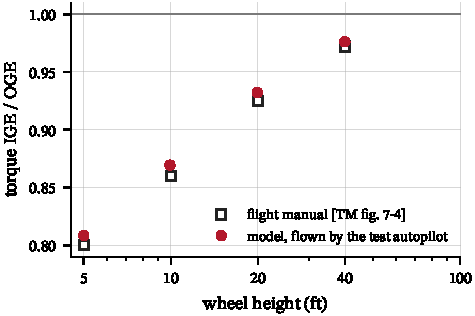
\includegraphics[width=\columnwidth]{ge.pdf}
\caption{Hover torque in ground effect relative to 100\,ft, model (flown by the test autopilot, 16\,000\,lb, sea level) and the operator's manual hover chart.}\label{fig:ge}
\end{figure}
\begin{table}[t]
\centering\small
\caption{Ground effect: hover torque relative to 100\,ft wheel height.}\label{tab:ge}
\Tab{ge}
\end{table}
With the test autopilot holding the height (Fig.~\ref{fig:ge}, Table~\ref{tab:ge}), the torque ratios are within \NGEmax{} of the
operator's manual at every height; flights in FlightGear with the same autopilot recorded 0.81, 0.87, 0.93 and 0.98.

\subsection{Control response}\label{sec:resp}
\begin{figure*}[t]
\centering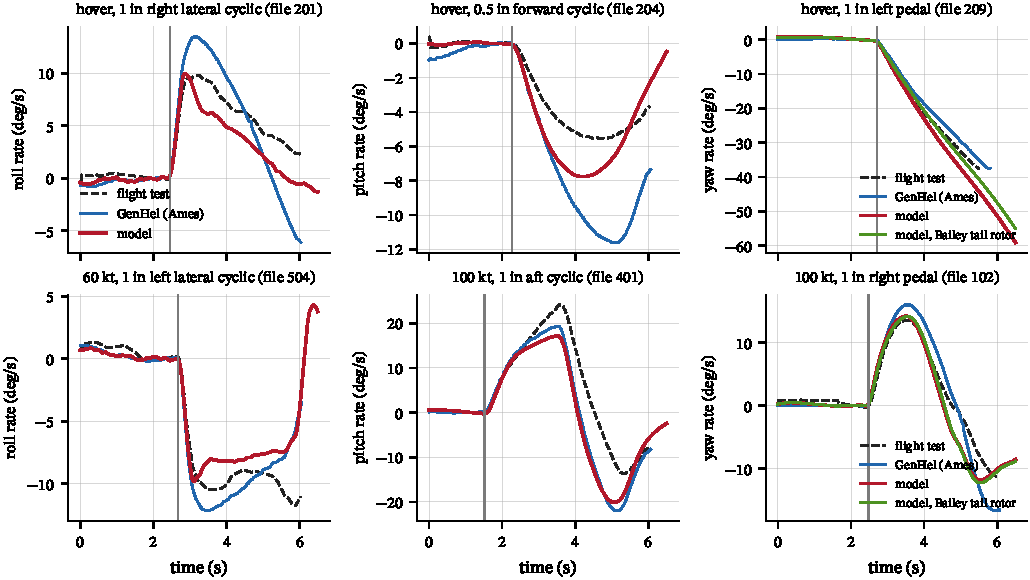
\includegraphics[width=\textwidth]{response.pdf}
\caption{On-axis rate after control steps with the SAS off (TM-88360 app.~D): flight test, GenHel as run at NASA Ames, and the model, as increments
from trim. The vertical line marks the input.}\label{fig:resp}
\end{figure*}
\begin{table*}[t]
\centering\small
\caption{Control responses (TM-88360 app.~D): peak on-axis rate in the 2.5\,s after the input, and the rms error of the rate against the
test over that interval (bold: model below GenHel). $^\dagger$The test pitch-rate trace of 509 could not be digitised reliably; excluded from the statistics.}\label{tab:resp}
\Tab{resp}
\end{table*}
Figure~\ref{fig:resp} shows six of the 17 cases and Table~\ref{tab:resp} all of them. The model's rms error is below GenHel's in
\NRbetter{} of \NRn{} cases, with a mean of \NRmod\,deg/s against GenHel's \NRgh\,deg/s. In hover the model sits between GenHel
and the test: GenHel's peak roll and pitch rates after cyclic steps are \NRghlo--\NRghhi\,\% larger than the test's, the model's
\NRmlo--\NRmhi\,\%. The model's peak yaw rate after the pedal step in hover is \NRped\,\% larger than the test's (rms error \NRpedrms\,deg/s,
GenHel \NRpedrmsgh). That case found a missing term: the rotor speed was integrated relative to the airframe from the torques alone, so a yaw
left the rotor's speed relative to the airframe unchanged and the rotor's inertia, a fifth of the airframe's, out of the yaw axis. With the
airframe's yaw acceleration in the rotor speed's equation (Section~\ref{sec:model}) a yaw to the left droops the rotor and the tail rotor with it,
and the governor's answer reaches the airframe as the drive torque's reaction; the hover pedal step's error fell from 5.5 to \NRpedrms\,deg/s.

Held in the hover, with rotors and governor settled, the model's yaw damping is $N_r$ = \NYdr\,s$^{-1}$: \NYdrtr{} from the tail rotor,
\NYdrmr{} from the main rotor's torque, which rises with the rotor's speed through the air, and \NYdrfin{} from the fin, whose share of the
tail rotor's jet grows as the tail swings into it. At the 1-kt condition of TM-85890 it gives $N_r$ = \NYdhbr\,s$^{-1}$, $N_v$ = \NYdhbv{} and
\NYdhbp\,rad/s$^2$ per inch of pedal, against $-$0.334, 0.0098 and 0.604 for that report's model. Flight identification of the UH-60A in hover
gave $N_r=-0.445$\,s$^{-1}$~\cite{flet}, and a first-order fit of the 209 test \NYawtestNr\,s$^{-1}$ for \NYawtestNp\,deg/s$^2$ per inch
(model \NYawmodNr{} and \NYawmodNp, GenHel \NYawghNr{} and \NYawghNp). The test's yaw acceleration, though, falls in the first half second
and then stays nearly constant for two seconds, and after the collective step of 212 the yaw rate keeps rising: shapes that no first-order
damping makes. The sideward-flight trims of 77-17, which test the same tail rotor physics in the steady state (Section~\ref{sec:xwind}),
agree with the model. The hover yaw damping is left open between these readings. The clearest deficiency is the aft cyclic step at 100\,kt: the test reaches \NQtest\,deg/s of pitch rate,
GenHel \NQgh\,deg/s, the model \NQmod\,deg/s. At 100\,kt both simulations also roll the wrong way after a pedal step, which neither
reproduces.

\subsection{The two tail rotor models}\label{sec:trcomp}
\begin{table}[t]
\centering\small
\caption{The blade-element and Bailey tail rotors against every test that involves the tail rotor. Pedal in per cent of travel or inches;
$^*$ not trimmed (the blade-element rotor at its limit).}\label{tab:tr}
\Tab{tr}
\end{table}
Table~\ref{tab:tr} collects the comparisons. The blade-element rotor makes more thrust per degree of pitch than Bailey's closed form,
some 0.4\,in of pedal at low speed, which brings it closer to the test in the hover, and it is about 2\,\% of pedal travel closer in level flight
and at zero sideslip. In crosswinds Bailey's rotor has the smaller pedal error, the blade-element rotor sitting to the right of the
high-altitude aircraft, and their tail rotor powers are alike. Bailey's rotor also has the smaller error after pedal steps; both are below GenHel's. The physical differences show at the edges of the
envelope: the blade-element rotor reaches its thrust limit from about 158\,kt, and in a left crosswind its blades meet the flow reversing through the disc.
For a pilot the difference is small; for the physics, the blade-element rotor is the one that can tell when it is being asked for too much.

\subsection{Stability derivatives}\label{sec:derivs}
\begin{table}[t]
\centering\small
\caption{Longitudinal derivatives at 100\,kt, 16\,400\,lb, FS\,360.4: TM-85890's model, and this model with the pitch bias actuator and stabilator active, and with
them held (rotor and airframe only). Per unit mass or pitch inertia; $\delta_e$ inch aft, $\delta_c$ inch up.}\label{tab:derivs}
\Tab{derivs}
\end{table}
The derivatives (Table~\ref{tab:derivs}) explain the weak pitch-up. The model's angle-of-attack stability is close to neutral, as
the aircraft's (79-24 found the static stability negative to neutral), but its $M_w$ of \NMwmod{} is a third of TM-85890's \NMwgh{}:
the stabilator's restoring moment nearly cancels the destabilising contributions of rotor and fuselage. $Z_w$ is \NZwmod{} against \NZwgh, and a Pitt--Peters wake gives the same, so it is not the
inflow model. $Z_q$ has the opposite sign to TM-85890's (\NZqmod{} against \NZqgh): in hinged-rotor theory pitch rate tilts the disc but does not change
its thrust in hub-plane axes, which the model follows. With the SAS on, 79-24 found a long-term aperiodic pitch divergence at 100\,kt
that the model does not show; it is stable with the pitch bias actuator on and close to neutral with it off.

% =====================================================================================================================
\section{Corrections found during validation}\label{sec:review}
The model is the result of several rounds of validation; the changes that the comparisons forced are listed here because each
removed a physical inconsistency rather than tuning a coefficient.
\begin{enumerate}
\item \emph{Rotor wake on the airframe in hover.} GenHel puts the in-plane part of the wake's velocity at the fuselage, fin and tail rotor along the body's
$x$ axis. The first version used the direction of the in-plane flow instead, which is undefined in hover: a drift of 0.05\,ft/s
swung 6\,ft/s of wash sideways onto the fin and tail rotor and kicked the aircraft in yaw. It now fades to the body axis below 5\,ft/s.
The hands-off hover with the SAS on became steady (heading within 0.7$^\circ$ in 30\,s, against 93$^\circ$ before).
\item \emph{Tip loss in the momentum balance} (Section~\ref{sec:power}): hover power was 4--9\,\% low and the figure of merit 0.03 high.
\item \emph{Accessory power}: a placeholder of 30\,hp was replaced by Sikorsky's 65.8\,hp, and an unsourced section drag increment of 0.002
by the 0.0012 of a tripped boundary layer.
\item \emph{Downwash correction terms}: GenHel's empirical wake-swirl forces on the empennage, defined in its motion module rather than the
empennage module, were missed at first; without them the aircraft trimmed with 1.4--2.5$^\circ$ of left bank at zero sideslip.
\item \emph{Test conditions}: the control responses were first replayed at the CG of fig.~B1. At the CG of table~C1, FS\,359.5 for the 100\,kt cases,
the aft-step pitch rate rose from 11.4 to 17.5\,deg/s.
\item \emph{Ground effect}: an earlier version scaled thrust; the effect is on the induced velocity, fitted to the hover chart and carried into
forward flight with the measured interference ratios.
\item \emph{Ground contact}: wheels alone let the fuselage sink through the ground when the aircraft rolled over, and JSBSim's wheel force diverges
as a strut lies along the ground. Structure contacts from the 3-D model and a rule that takes the wheels out of play beyond 60$^\circ$ of tilt fixed both.
\item \emph{Main rotor wake at the tail}: GenHel gives the tail rotor the empennage's wash, and the first version also turned the in-plane
part with the flight path, so that in sideward flight the tail rotor met a crosswind 1.4 times the real one and, through its cant, a phantom
climb from 2.1 times the inflow of downwash. The pedal swing between winds from the right and from the left was nearly twice the test's.
The ring wake (Section~\ref{sec:model}) at the tail rotor, fin and stabilator brought the crosswind pedal error from \NXGped{} to
\NXBped\,in rms and the longitudinal cyclic error from \NXGlon{} to \NXBlon\,in, without changing forward flight.
\item \emph{Trims off the nose}: a trim in angle of attack and sideslip fails at 90$^\circ$ off the nose; the attitudes are now the trim
variables there.
\item \emph{Rotor speed and the airframe's yaw}: the rotor speed was integrated relative to the airframe from the torques alone, as if the
airframe's yaw did not concern the rotor (Section~\ref{sec:resp}). With the term the hover pedal step's yaw-rate error fell from 5.5 to
\NRpedrms\,deg/s.
\item \emph{Fin blockage}: an intermediate version scaled the tail rotor wake's velocity at the fin to Sikorsky's 20.4\,\% blockage. That made
the fin anti-damping in yaw ($+$0.06\,s$^{-1}$ in the hover, against $+$0.02 unscaled) and was removed.
\end{enumerate}

% =====================================================================================================================
\section{Assessment}\label{sec:assess}
\begin{table}[t]
\centering\small
\caption{Summary: \ok{} within the test's scatter, \pok{} partly, \nok{} not reproduced.}\label{tab:score}
\begin{tabularx}{\columnwidth}{@{}>{\raggedright\arraybackslash}Xc@{}}
\toprule
Trim controls and attitudes, 50--139\,kt & \ok \\
Trim at 162\,kt (collective, lateral cyclic, pedal) & \pok \\
Lateral-directional trim at zero sideslip & \ok \\
Bank change between climb and descent & \pok \\
Hover power, OGE and in ground effect & \ok \\
Rotor figure of merit & \ok \\
Tail rotor power in hover & \pok \\
Pedal and longitudinal cyclic hovering in a wind, 10--40\,kt & \pok \\
Tail rotor power hovering in a wind & \pok \\
Tail rotor power in level flight: low speed and 150\,kt \ok, cruise \nok & \pok \\
Cruise power (one test \ok, the other \nok) & \pok \\
Responses to cyclic, collective, pedal in hover and at 60\,kt & \ok \\
Yaw damping in hover & \pok \\
Pitch-up after an aft step at 100\,kt & \pok \\
Roll after a pedal step at 100\,kt & \nok \\
Long-term pitch divergence with SAS (79-24) & \nok \\
\bottomrule
\end{tabularx}
\end{table}
Table~\ref{tab:score} summarises. The model reproduces the Black Hawk's trim, its hover and ground-effect power and its short-term
responses at least as well as GenHel, from which it was derived, and in hover better. Its open items share one direction: in
pitch at speed the model is too stable. A third of TM-85890's $M_w$, too small a pitch-up after an aft step and no long-term divergence
point to the same missing destabilising moment, and Section~\ref{sec:derivs} locates it in the balance of rotor, fuselage and stabilator rather than in
any single term. The other open items are the cruise power against one of the two tests, the tail rotor's power (low in the hover
against one test, high in cruise against another), the hover yaw damping, the anti-torque at the top speed, and the lateral moment per inch
of cyclic. Retreating-blade stall limits the
model at high thrust and speed ($C_T=0.009$ above $\mu=0.28$); blade torsion is not modelled, and dynamic stall only as a tail rotor experiment.

% =====================================================================================================================
\section{Conclusions}\label{sec:concl}
\begin{itemize}
\item A blade-element model of the UH-60A with individual blades, a finite-state dynamic wake, GenHel's airframe and control laws, and
engines runs in plain JSBSim, generated from data. It is the flight model of the FlightGear UH-60A.
\item Against the US Army flight tests it reproduces level-flight longitudinal cyclic and collective within \NBmaxlon\,\% of travel up to 162\,kt,
hover power at \NHmin--\NHmax{} of the measured over the test's range, ground effect within \NGEmax{} and the SAS-off control responses with a smaller error than GenHel.
\item Applying tip loss to the momentum balance as well as the lift brings the rotor's figure of merit and the aircraft's hover power into line with
the measurements; GenHel's lift-only tip loss leaves the induced power ideal.
\item Where the main rotor's wake goes matters at the tail: GenHel's interference factors, measured with the wake blown aft, put it on the
tail rotor and stabilator in any wind. A ring-vortex wake that follows the wind, with the fin in the tail rotor's own wake, halves the error
of the pedal hovering in winds from every direction without changing forward flight.
\item A blade-element tail rotor reproduces the tests at least as well as GenHel's closed form and shows its thrust limit from about 158\,kt,
where the closed form has none; that the aircraft flew 162\,kt with less tail rotor pitch points to anti-torque the model lacks at the top speed.
\item The rotor's angular momentum about its shaft is its own: a rotor speed taken relative to the airframe has to follow the airframe's yaw.
The term was missing, and with it the yaw after a hover pedal step comes close to the test's.
\item The pitch stability at speed is too strong and the cruise power against the 77-17 data too high; both are documented, not tuned away.
\end{itemize}

\begin{thebibliography}{99}\small
\bibitem{gh} Sikorsky Aircraft, \emph{UH-60A Black Hawk Engineering Simulation Program, vol.~I: Mathematical Model}, NASA CR-166309, 1981.
\bibitem{hb} NASA Ames Research Center, \emph{A Mathematical Model of the UH-60 Helicopter}, NASA TM-85890, 1984.
\bibitem{bal} NASA Ames Research Center, \emph{Validation of a Real-Time Engineering Simulation of the UH-60A Helicopter}, NASA TM-88360, 1987.
\bibitem{kap} Sikorsky Aircraft, \emph{UH-60 Black Hawk Engineering Simulation Model Validation and Proposed Modifications}, NASA CR-177360, 1986.
\bibitem{a7924} US Army Aviation Engineering Flight Activity, \emph{Validation Flight Test of UH-60A for Rotorcraft Systems Integration Simulator}, USAAEFA Project 79-24, DTIC ADA125428, 1982.
\bibitem{a7717} US Army Aviation Engineering Flight Activity, \emph{Airworthiness and Flight Characteristics Evaluation, UH-60A (Black Hawk) Helicopter}, USAAEFA Project 77-17, DTIC ADA132068, 1981.
\bibitem{a8324} US Army Aviation Engineering Flight Activity, \emph{Airworthiness and Flight Characteristics Test of a Sixth Year Production UH-60A}, USAAEFA Project 83-24, DTIC ADA180181, 1985.
\bibitem{a85} US Army Aviation Engineering Flight Activity, UH-60A test report, DTIC ADA180404.
\bibitem{bous} NASA Ames Research Center, \emph{Aerodynamic Characteristics of SC1095 and SC1094 R8 Airfoils}, NASA TP-2003-212265, 2003.
\bibitem{nacaexp} \emph{A critical assessment of wind tunnel results for the NACA 0012 airfoil}, AGARD CP-429, 1987.
\bibitem{lrta} \emph{Full-scale wind tunnel test of the UH-60A rotor (NASA Ames Large Rotor Test Apparatus)}, American Helicopter Society 58th Annual Forum, 2002.
\bibitem{perf} \emph{Performance analysis of a utility helicopter with standard and advanced rotors}, Journal of the American Helicopter Society 49(3), 2004.
\bibitem{heyson} NASA, \emph{Ground effect for lifting rotors in forward flight}, NASA TN D-234, 1960.
\bibitem{metu} Middle East Technical University, M.Sc.\ thesis on rotor inflow models (Peters--He finite-state wake).
\bibitem{tm} Department of the Army, \emph{Operator's Manual, UH-60A and UH-60L Helicopters}, TM 1-1520-237-10, with change 10.
\bibitem{t700} NASA, \emph{A Rotorcraft Flight/Propulsion Control Integration Study}, 1987.
\bibitem{johnson} \emph{Rotorcraft Aeromechanics}, Cambridge University Press, 2013, section 3.6.
\bibitem{flet} NASA Ames Research Center, \emph{A Model Structure for Identification of Linear Models of the UH-60 Helicopter in Hover and Forward Flight}, NASA TM 110362, 1995.
\bibitem{a87} US Army Aviation Engineering Flight Activity, UH-60A test report (External Stores Support System), DTIC ADA181947.
\bibitem{gorm} Boeing Vertol, \emph{A Mathematical Model of Unsteady Aerodynamics and Radial Flow for Application to Helicopter Rotors}, USAAMRDL TR 72-67, 1973.
\bibitem{jsbsim} JSBSim Development Team, \emph{JSBSim: an open-source flight dynamics model}, version 1.3.3.
\end{thebibliography}
\end{document}
